\documentclass[oneside]{report}
\usepackage[T1]{fontenc}
\usepackage[utf8]{inputenc}
\usepackage[frenchb]{babel}
\usepackage{graphicx}
\usepackage[margin=2cm]{geometry}
\usepackage{fancyhdr}
\usepackage{changepage}
\usepackage{etoolbox}
\usepackage{xcolor}
\usepackage{titlesec}

\titleformat{\chapter}[display]
{\normalfont\huge\bfseries}{}{20pt}{\Huge}

\titlespacing*{\chapter}{0pt}{0pt}{0pt}
\graphicspath{ {images/} }


\author{Nathan JANCZEWSKI, Léo BERGEROT, Loic HUSSON, Youness LOUCIF,\\ Alexandre QUILLET, Jonathan PAUGOIS }

\usepackage{etoolbox}
\patchcmd{\chapter}{plain}{fancy}{}{}

\newcommand{\writecol}[1] {
	\subitem{\textcolor[HTML]{#1}{\# #1}}
}

\newcommand{\indentunder}{1.5cm}
\begin{document}
	\begin{titlepage}
		\centering		
		
\includegraphics[scale=2]{logo}
		\vspace{5cm}
		{\par\scshape\Huge Cahier des charges \par}
		\vspace{0.5cm}
		{\par\scshape\Large Site web pour l'Université Pan Africaine\par}
		\vspace{10cm}
		{\par Université Pan Africaine (UPA)\par}
		{\par Site web \par}
		{\vfill}
		{\par Contact: \par}
		{\par\small Mme GUESSOUM Zahia\par}
		{\par zahia.guessoum@univ-reims.fr \par}
	\end{titlepage}		

\pagestyle{fancy}
\fancyhf{}
\rhead{
\includegraphics{logo}}
\lhead{Cahier des charges}

	\tableofcontents
	
	\chapter{Présentation de l'École}
	{
		
		\par Les instituts des Universités Pan Africaines ont pour but d’améliorer la qualité d'apprentissage des sciences et technologies.
		\vspace{1cm}
		\par C’est en 2003 à Johannesbourg lors de la première Conférence ministérielle sur l’environnement que naît l’idée de créer un réseau destiné à promouvoir et à faciliter la mobilité des étudiants comme des enseignants, harmoniser les programmes universitaires, répondre aux défis auxquels le continent le continent africain devra faire face et améliorer l’attractivité des études en Afrique.
		\vspace{1cm}
		\par Une des antennes de cette Université est l’Institut de Université PanAfricaine pour les Sciences de l’Eau et de l'Énergie (y compris le changement climatique) (PAUWES), institué lors de la Commission de l’Union Africaine réunie en 2008, à Tlemcen au Nord-Ouest de l’Algérie. 
		\vspace{1cm}
		\par Elle offre deux programmes d’études supérieures :
		\begin{itemize}
			\item{Master en Science de l’énergie}
			\item{Master en Science de l’eau}
		\end{itemize}
	}
	\chapter{Présentation du projet}
	{
		\par Rendre le site web plus utile pour:
		\begin{itemize}
			\item{L'administration}
				\subitem{Inscrire les nouveaux étudiants}
				\subitem{Gère le dossier personnel des étudiants}
				\subitem{Accède à la base de donnée de tous les étudiants}
				\subitem{Mettre à jour les emplois du temps}
				\subitem{Relever les abscences des étudiants}
			\item{Les étudiants}
				\subitem{Accès en ligne aux cours}
				\subitem{Accès à l'emploi du temps personnel}
				\subitem{Messagerie}
				\subitem{Modifier les données personnelles}
				\subitem{Consulter les notes}
			\item{Les enseignants}
				\subitem{Déposer les cours en ligne}
				\subitem{Messagerie}
				\subitem{Consulter son emploi du temps}
				\subitem{Gestion des notes}
				\subitem{Relever les abscences des étudiants}
		\end{itemize}
		\vspace{1cm}
		\par\underline{Ce qui ne va pas}:
		\vspace{.5cm}
		\begin{adjustwidth}{\indentunder}{}
		\begin{itemize}
			\item Le site actuel est très utile à but informatif, mais ne permet aucune gestion de l'antenne Algérienne.
			\item Il n'offre aucune plus-value aux étudiants suivants déjà les cours à l'université, et encore moins aux professeurs.
			\item Il y a deux carroussels présents sur toutes les pages prenant une place considérable, forçant ainsi l'utilisateur à descendre sur la page.
			\item Le comportement de ceux-ci est très aléatoire
			\item La présence de deux menu porte confusion
			\item Pas d'attribut ALT sur les images
			\item Certaines pages dans les mauvaises catégories (Welcome dans About par exemple)
		\end{itemize}
		\end{adjustwidth}
	\vspace{1cm}
	\par\underline{Ce qui va}:
		\vspace{.5cm}
		\begin{adjustwidth}{\indentunder}{}
		\begin{itemize}
			\item L'utilisation du framework Bootstrap garantie une adaptabilité et le fonctionnement sur une grande variété de navigateurs.
			\item Les informations sur le sites sont correctes
			\item Volonté de minimiser les couleurs afin de garantir un accès aux malvoyants
		\end{itemize}
		\end{adjustwidth}
	
		\section{Comité de pilotage}
		{
			\par L’équipe attitré au projet utilise la méthode \textit{SCRUM}. Cela veut dire que le développement se découpera en sprints, période sur lequel l’équipe planifiera les fonctionnalités qui devront être implémentées, qui se conclura sur une démonstration au client qui pourra alors vérifier le respect du cahier des charges à son gré ainsi que la validation du graphisme et du contenus.
			\vspace{.5cm}
			\par Si le client le souhaite, la validation de l’ergonomie sera effectuée en testant sur des personnes externes (Hors scolarité pour la recherches d’informations, ainsi qu’étudiants et professeurs pour leurs parties respectives)

		}
		\section{Objectifs du site}
		{
			Le site est d’une part un site d’informations à destination d’élèves souhaitant intégrer une université afin de décrire le fonctionnement de celle-ci, mais aussi un support de cours et communications entre étudiants et professeurs de l’université.
		}
		
		\section{Les cibles (À qui s'adresse le site ?)}
		\par Le sites s'adresse d'une part aux futur étudiants recherchant des informations sur les diverses formations, d'autre part il s'adresse à l'administration de l'Université, aux professeurs ainsi qu'aux élèves qui auront un accès avec plus de fonctionnalités.
		\section{Plan du site (Arborescence)}
		\par L'arborescence est la suivante:\\
		\begin{center}
			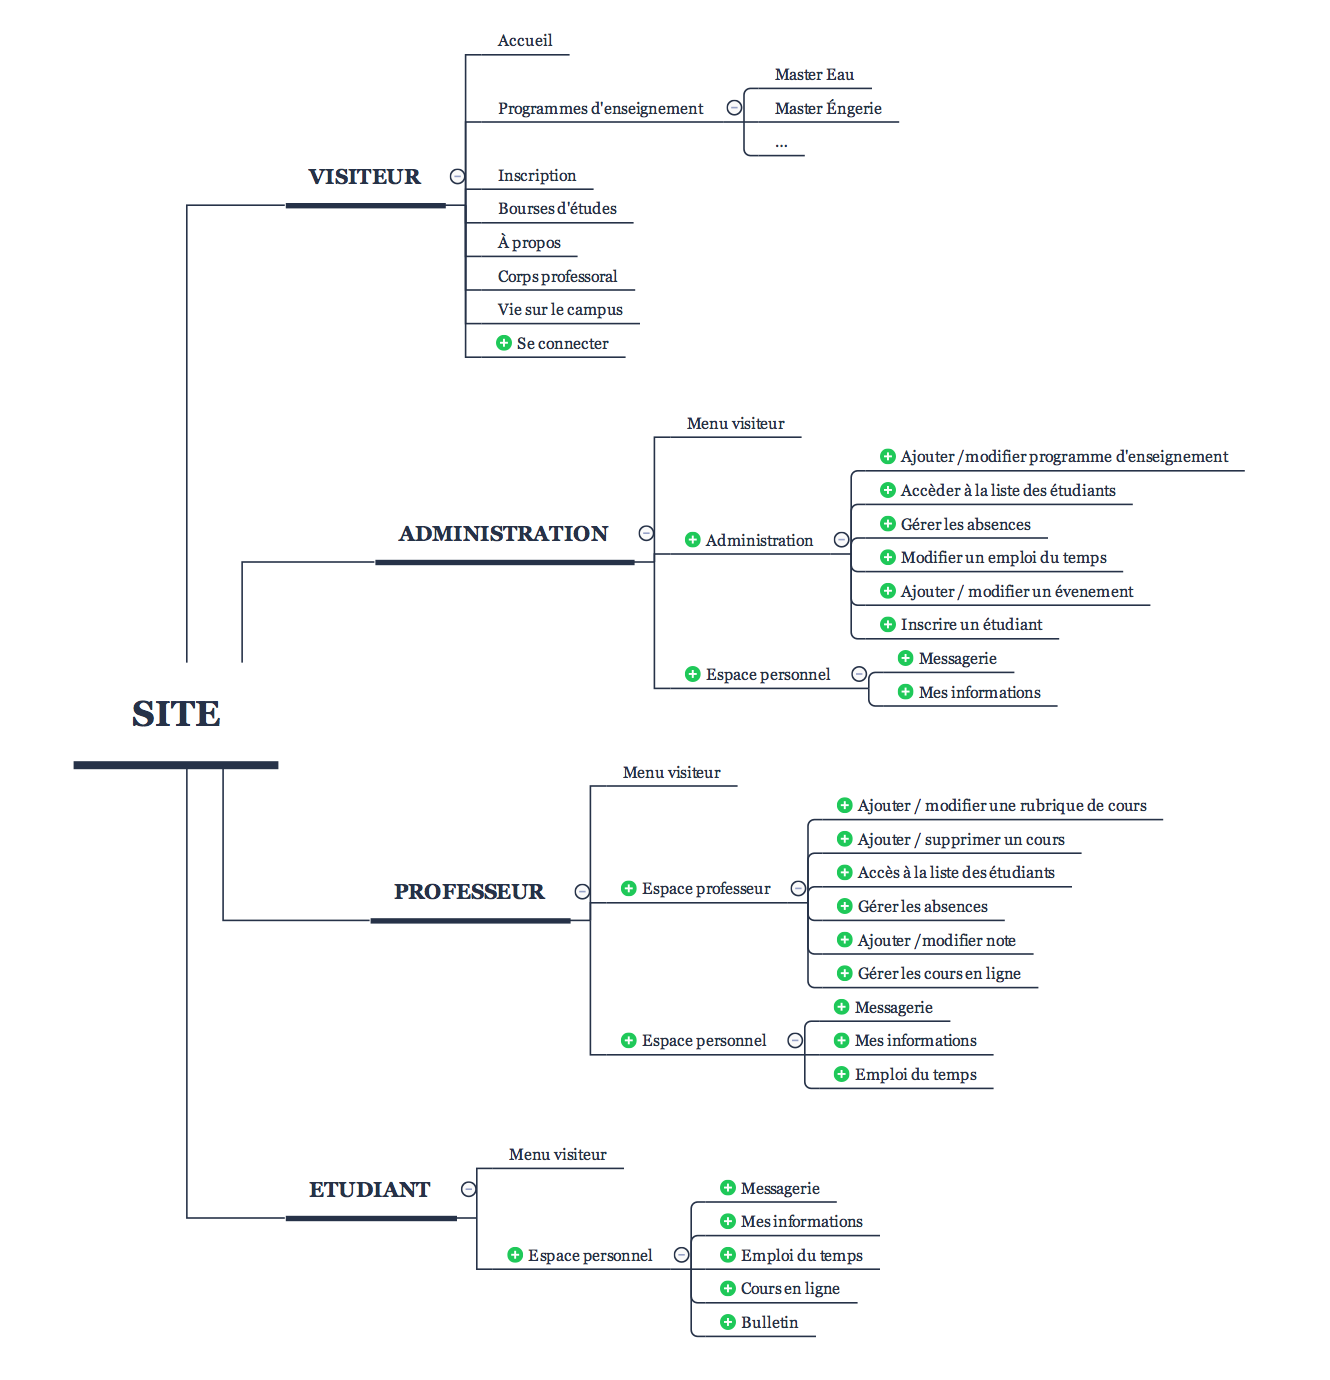
\includegraphics[scale=1.5]{arborescence}
		\end{center}
		\section{Contenus}
		{
			\par Le site reprendra les diverses informations accessibles sur le site actuel, qui seront re-triées afin d’obtenir une ergonomie plus accessible, mais permettra tout de même de modifier ce qui à été inclu, celui-ci se comportant comme un CMS (Ou SGC, système de gestion de contenu)
		}

		\section{Fonctionnalités}
		{
			\par Diagramme UML des fonctionnalités du site web:\\
			\begin{center}
				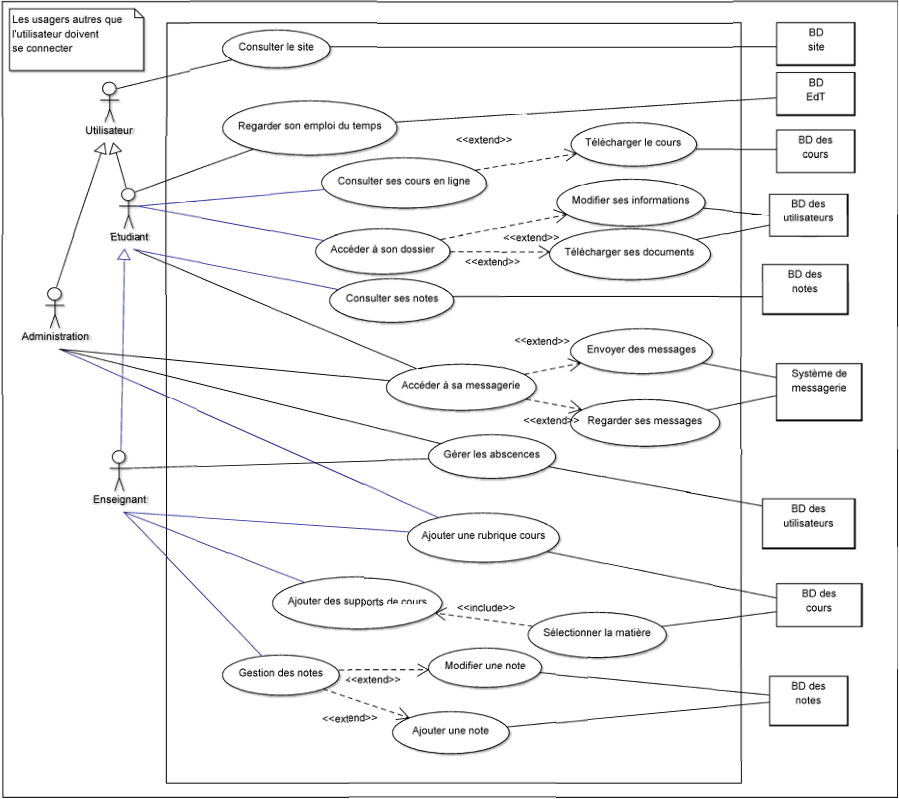
\includegraphics[scale=1.5]{uml_base}
				\\
				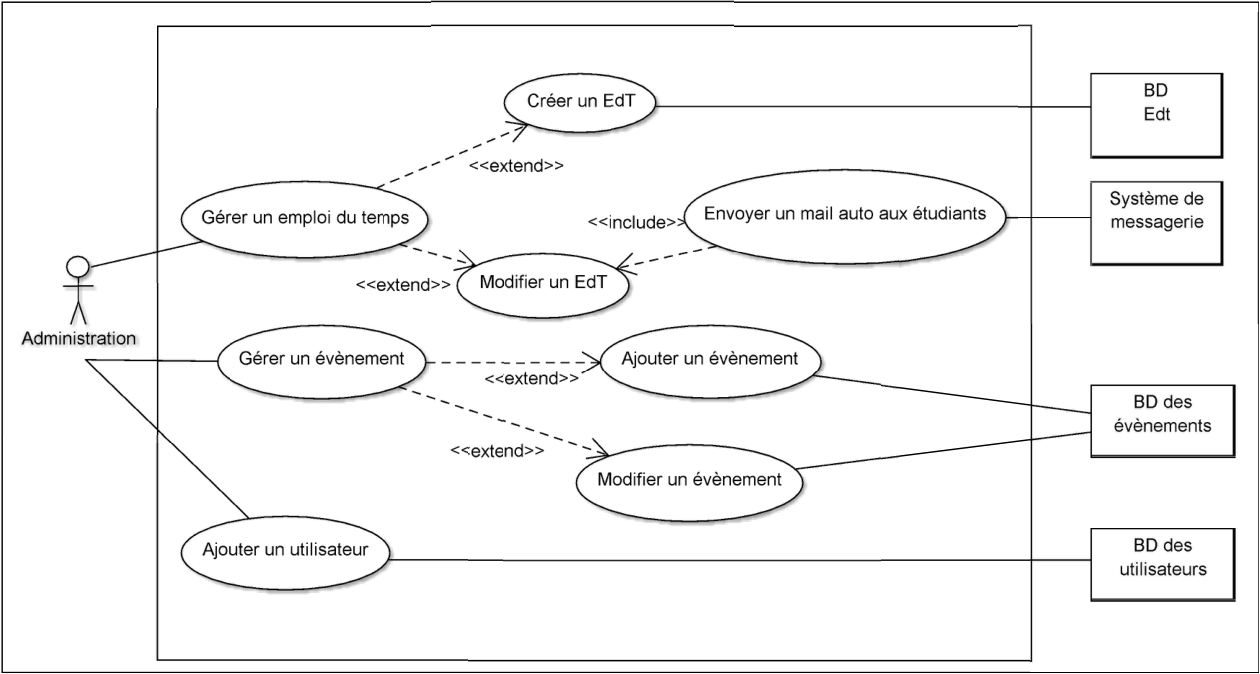
\includegraphics[scale=1.5]{uml_admin}
			\end{center}
		}
		\section{Langues}
		{
			\par Le site sera conçu avec un système de traduction permettant ainsi au besoin d'ajouter d'autres langues que les deux de bases qui seront Anglais et Français.
		}
	}
	\chapter{Prestations attendues}
	{
		\section{Charte graphique}
			\begin{itemize}
				\item{Couleurs}
					\writecol{639D35}
					\writecol{040707}
					\writecol{868786}
					\writecol{005899}
					\subitem{\# FFFFFF (Blanc pure)}
				\item{Typographie: Roboto Sans-Serif}
				\item{Logo}
					\subitem{
\includegraphics[scale=2]{logo}}
			\end{itemize}
		\section{Création et récupération de contenus}
		{
			\par Le contenus déjà disponible se compose de diverses photos dont les auteurs sont:
			\vspace{.5cm}
			\begin{itemize}
				\item Tlemcen University
				\item Mr Hefhaf/Tlemcen University
				\item Michael Gajo/GIZ
				\item michaeljung/Fotolia
				\item paulmz/Fotolia
				\item Piotr Pakuła/Fotolia
				\item Zurijeta/Shutterstock
				\item john michael evan potter/Shutterstock
				\item PhotoSky/Shutterstock
				\item bikeriderinlondon/Shutterstock
				\item Tyler Olson/Shutterstock
			\end{itemize}
			\vspace{.5cm}
			\par Nous nous baserons sur le contenu déjà utilisé et nous n'aurons pas besoin de contenus supplémentaires.
			\vspace{.5cm}
		}
		\section{Développement}
		\par Pour gérer correctement l’automatisation de chaque tâches, il sera nécessaire d’utiliser de la programmation orientée objet (PHP), les information seront stocké dans une base de donnée (SQL).
		\par
		\begin{itemize}
			\item Gestion automatique d’ajout des formations
			\item Gestion de la modification de l’emploie du temps avec envoie automatique d'e-mail pour prévenir les personnes
			\item Moteur de recherche interne au site
			\item Gestion automatique d’ajout et modification des événements (actualitées)
			\item Gestion ajout et modification des informations personnels(dossier étudiant, dossier professeur)
			\item Gestion d’ajout des cours en lignes et téléchargement de ceux-ci
			\item Gestion des absences
		\end{itemize}
		\section{Dépot du nom de domaine et adresses mail}
		{
			\par Le nom de domaine "\textit{http://pauwes.univ-tlemcen.dz/}" étant déjà déposé, aucun coût supplémentaires seront à prévoire à ce niveau la. Cependant la configuration du serveur mail peut-être à prévoire en fonction de la configuration actuelle de l'hébergeur.
		}
		\section{Hébergement}
		\section{Référencement}
		\section{Mises à jour}
		{
			\par Le site étant développé comme un CMS, il a parmis ses objectifs d’être dynamique, ainsi l’équipe administrative pourra modifier le contenu, les pages et menus depuis l’interface destinée à être simple d’utilisation.
			\par Cependant, un contrat de maintenance pourra être mis en place si un ajout de fonctionnalités est susceptible d’être demandé dans le futur.
		}
		\section{Statistiques de connections}
	}

	\chapter{Réponse attendue}
	{
	
	}

	\chapter{Planning prévisionnel}
	{
	
	}

	\chapter{Budget}
	{
		
	}
\end{document}
